\subsection{Android Application}
\label{sec:android-application}

The main role of the Android application in this system is to receive ultrasonic waves using microphones on the smartphones. Therefore, the ultrasonic signal range is required to satisfy two conditions. The signal should not be heard by humans, at the same time it should be heard by microphones. The audible range of frequency for humans is between 20Hz and 20kHz, while most microphones on smartphones support sampling rate of 44.1kHz, which is greater than Nyquist rate relative to the highest human audible frequency, 40kHz, to avoid aliasing of the signal. However, as 44.1 kHz is still higher than the Nyquist rate, we can easily speculate that the smartphones are theoretically capable of recording the frequency range between 0 Hz to 22.05 kHz without aliasing, although it will become more difficult to differentiate signals when the frequency gets closer to either of two extremes. The frequency band ranging from 20 kHz to 22.05 kHz satisfies the two conditions mentioned above; this band is not hearable for humans but still hearable for smartphones. However, according to our experiments, the received signal strength becomes too weak to be feasible around the frequency of 21.0 kHz when the frequency goes higher.

The amount of computation gets overly intensive when the number of points in fast Fourier transform (FFT) exceeds 2048. Although the more number of points in FFT gives us the finer granularity to represent data using ultrasound signals, increasing the number of points in FFT requires more computations, which can be a burden for embedded systems such as smartphones. After carrying out experiments related to the proper number of points in FFT, we concluded that 2048 points would be a limit for current smartphones since 4096 point FFT slightly slowed down the response time of recent Android devices like Samsung GalaxyS 3 and Google Nexus 7. 2048 point FFT gives us a feasible resolution of approximately 10.76 Hz per each point so we have about 94 points from 20.0 kHz to 21.0 kHz. It is not possible to fully utilize these points as bits because there is noise in FFT results around the target frequencies due to limitation of precision in sound generation and FFT. Considering the interference caused by neighboring signals, leaving space in frequencies between signals would be proper to obtain clear data from decoding. Therefore, we divided this range of frequency between 20.0 kHz and 21.0 kHz into eight intervals removing 21.0 kHz frequency from the range in order to increase correctness in decoding, assigning 8 bits at between 20.0 kHz and 20.875 kHz as demonstrated in Fig.\,\ref{fig:data_representation}.

To decode room ID from FFT results, differentiating the actual signal value from noise and interference caused by ultrasound generators, environments and neighboring signals. Before taking interference by neighboring signals into consideration, the noise by the generator should be eliminated. Even though the created wav signal by Matlab is quite clear, it might involve some noise from speakers and circuits. If the application always try to choose the FFT result at the exact target frequency it will still have chances to select a signal weaker than what is actually necessary for decoding as shown in Fig.\,\ref{fig:fft_results} box (a). Selecting maximum value among the results which are right beside to the target frequency rather than just picking up the value at the exact frequency can remove this possibility, and we call this value as a “signal value”. The easiest way to detect a signal is to compare the signal value with an absolute value and determine that there is a signal if the signal value is greater than absolute value. However, this method does not work because the signal at neighboring frequencies will affect the FFT result of the target frequency making it hard to differentiate the real signal and the fake signals caused by noise of neighboring signals such as in Fig.\,\ref{fig:fft_results} box (b). To differentiate actual signals from noise and interference of neighboring signals, just comparing the signal value with an absolute value is not sufficient. This tricky problem can be solve by setting “reference values” to be compared with the signal value. Even though there is noise by the signals around the signal value, they tend to be diminished as they get further from its target frequency. Hence, if the signal value is greater than FFT results around the signal value, then we can conclude that there is a signal. The reference values are set as the sum of the FFT results apart from the target frequency by three points scaled by a predefined factor and a base noise, which is a threshold or an absolute value that is set according the target frequency. Since the received signal strength becomes weaker as the frequency increases, the threshold is set to decrease as the target frequency increases.

The Android application is able to determine whether there is a signal by comparing the signal value to the reference values as explained above. But there is one more problem left that needs a solution, the decoded value using this method is still unstable changing frequently as time passes. This can lead to wrong reading or too frequent fluctuation of room ID that makes it difficult to localize the target.  The problem can happen especially when the target person with a phone enters a room with an ultrasound generator. The application employs an exponential moving average denoted in \ref{eqn:1} to stabilize the decoded result and wait until the decoded value after the exponential moving average becomes constant to avoid frequent fluctuation when the localization process begins right after the target enters a room with an ultrasound generator.

\begin{equation}
t>1, s_t=\alpha \cdot y_t+(1-\alpha)\cdot s_{t-1}
\label{eqn:1}
\end{equation}
By using this two-level filtering method, we could obtain almost perfectly clear room ID results.
\ref{eqn:1}

This application also provides additional features to show the target's location depending on the user's selection. Users can choose to share their position on a map through the sMAP server using HTTP POST by sending the localization result to a dedicated server. By setting the user's name on the application interface, the users can publish their positions on the map provide by the server so that other people can identify where they are. The users may keep their location information secret without publishing their position to the public for their privacy. In this case, the application uses a map embedded to the application to show the location of the target without specifying the user's name. The user interface of Android application is also illustrated in Fig.\,\ref{fig:app_interface}. The space between check boxes and a start/stop button can be used to show either the private map or FFT results in graph as shown in leftbottom of the Fig.\,\ref{fig:app_interface}.

\begin{figure}
  \centering
  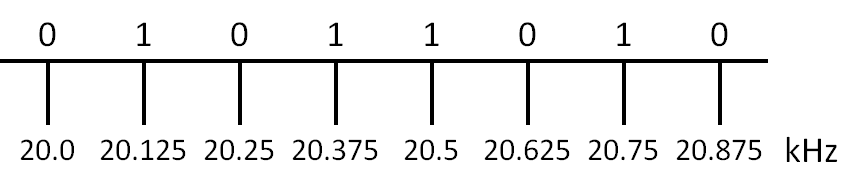
\includegraphics[width=0.8\columnwidth]{data_representation.png}
  \caption{Data representation on frequency band ranging from 20.0 kHz to 20.875 kHz}
  \label{fig:data_representation}
\end{figure}

\begin{figure}
  \centering
  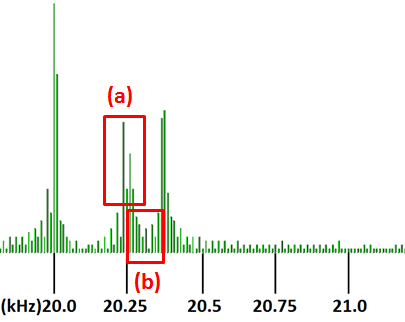
\includegraphics[width=0.7\columnwidth]{fft_results.png}
  \caption{Results of 2048 point FFT on Android application}
  \label{fig:fft_results}
\end{figure}

\begin{figure}
  \centering
  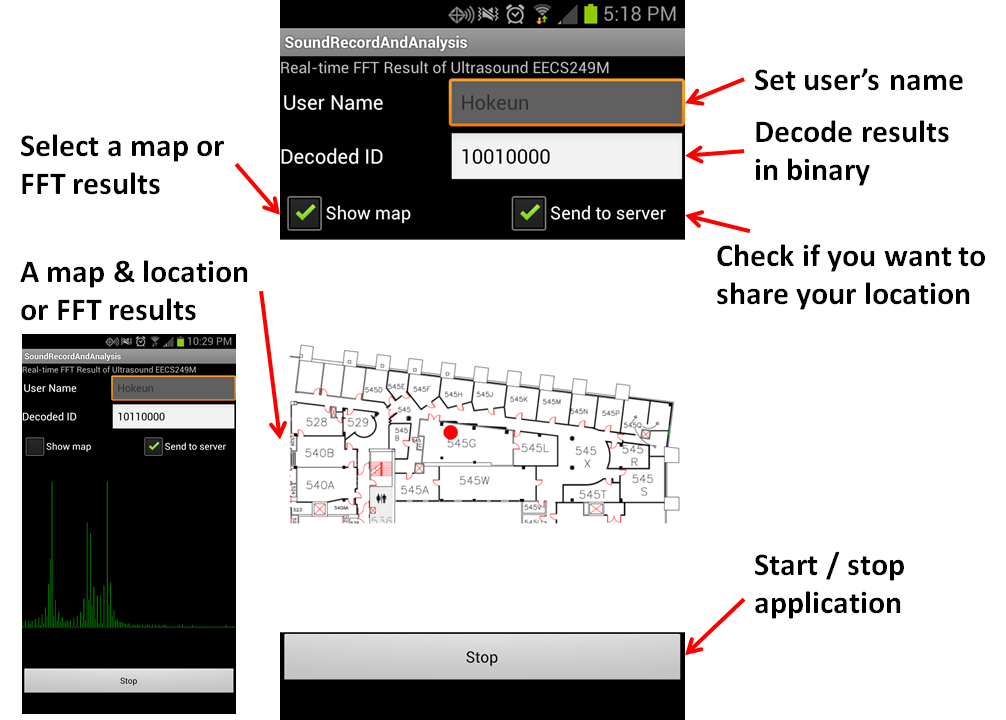
\includegraphics[width=\columnwidth]{app_interface.png}
  \caption{User interface of Anrdoid application}
  \label{fig:app_interface}
\end{figure}

%% Master
%%% Local Variables: 
%%% mode: latex
%%% TeX-master: "ee149"
%%% End: 
